% Template for Cogsci submission with R Markdown

% Stuff changed from original Markdown PLOS Template
\documentclass[10pt, letterpaper]{article}

\usepackage{cogsci}
\usepackage{pslatex}
\usepackage{float}
\usepackage{caption}

% amsmath package, useful for mathematical formulas
\usepackage{amsmath}

% amssymb package, useful for mathematical symbols
\usepackage{amssymb}

% hyperref package, useful for hyperlinks
\usepackage{hyperref}

% graphicx package, useful for including eps and pdf graphics
% include graphics with the command \includegraphics
\usepackage{graphicx}

% Sweave(-like)
\usepackage{fancyvrb}
\DefineVerbatimEnvironment{Sinput}{Verbatim}{fontshape=sl}
\DefineVerbatimEnvironment{Soutput}{Verbatim}{}
\DefineVerbatimEnvironment{Scode}{Verbatim}{fontshape=sl}
\newenvironment{Schunk}{}{}
\DefineVerbatimEnvironment{Code}{Verbatim}{}
\DefineVerbatimEnvironment{CodeInput}{Verbatim}{fontshape=sl}
\DefineVerbatimEnvironment{CodeOutput}{Verbatim}{}
\newenvironment{CodeChunk}{}{}

% cite package, to clean up citations in the main text. Do not remove.
\usepackage{cite}

\usepackage{color}

% Use doublespacing - comment out for single spacing
%\usepackage{setspace}
%\doublespacing


% % Text layout
% \topmargin 0.0cm
% \oddsidemargin 0.5cm
% \evensidemargin 0.5cm
% \textwidth 16cm
% \textheight 21cm

\title{Postural developments mediate children's visual access to social
information}


\author{{\large \bf Alessandro Sanchez} \\ \texttt{sanchez7@stanford.edu} \\ Department of Psychology \\ Stanford University \And {\large \bf Bria Long} \\ \texttt{bria@stanford.edu} \\ Department of Psychology \\ Stanford University \And {\large \bf Ally Kraus} \\ \texttt{allison.m.kraus@gmail.com} \\ Department of Psychology \\ Stanford University \And {\large \bf Michael C. Frank} \\ \texttt{mcfrank@stanford.edu} \\ Department of Psychology \\ Stanford University}

\begin{document}

\maketitle

\begin{abstract}
The ability to process social cues--including eye gaze--is a critical
component of children's early language and cognitive development.
However, as children reach their first birthday, they begin to locomote
themselves, walking and exploring their visual environment in an
entirely new way. How do these postural and locomotive changes affect
children's access to the social information relevant for word-learning?
Here, we explore this question by using head-mounted cameras to record
infants' (8-16 months of age) egocentric visual perspective and use
computer vision algorithms to detect the proportion of faces and wrists
in infants' environments. We find that infants' posture and orientation
to their caregiver largely mediates their access to social information,
suggesting that postural and locomotive developments play a significant
role in the emergence of children's linguistic and social capacities.
Broadly, we suggest that the combined use of head-mounted cameras and
the application of new computer vision techniques is a promising avenue
for understanding the statistics of infants' visual and linguistic
experience.

\textbf{Keywords:}
social cognition; face-perception; infancy; locomotion; head-cameras;
deep learning
\end{abstract}

\section{Introduction}\label{introduction}

Children are deeply engaged in learning from others (Csibra \& Gergely,
2009; Meltzoff, 2007) and attend to the social information in their
environment from their earliest days. Even newborns tend to prefer to
look at faces with direct vs.~averted gaze (Farroni, Csibra, Simion, \&
Johnson, 2002) and young infants follow overt gaze shifts (Gredebäck,
Fikke, \& Melinder, 2010; Gredebäck, Theuring, Hauf, \& Kenward, 2008).
Further, when infants free-view videos, they tend to look mostly at
faces at the expense of other visual information--though older infants
start to look towards people's hands and the actions they are performing
(Frank, Amso, \& Johnson, 2014; Frank, Vul, \& Saxe, 2012).

However, as children are learning from others around them, their view of
the world is also radically changing (K. Adolph \& Berger, 2007).
Infants' motor abilities improve dramatically near the end of the first
year of life, allowing them to locomote independently. These motor
changes have significant consequences for what children see; crawling
and walking infants simply have different views of the world. For
example, during spontaneous play in a laboratory playroom, toddlers are
more likely to look at the floor while crawling than while walking (J.
Franchak, Kretch, Soska, \& Adolph, 2011); in general, walking infants
tend to have full visual access to their environment and the people in
it, while crawling infants do not (K. S. Kretch, Franchak, \& Adolph,
2014).

One possibility is that these motor improvements have strong
developmental cascades, impacting children's emerging social, cognitive,
and linguistic abilities (Iverson, 2010). Indeed, these postural changes
also impact how children interact with their mothers; walking
(vs.~crawling) infants make different kinds of object-related bids for
attention from their mothers and tend to hear more action directed
statements (e.g., ``open it'') (Karasik, Tamis-LeMonda, \& Adolph,
2014). Further, in an observational study, Walle \& Campos (2014) found
that children who were able to walk had both higher receptive and
productive vocabularies. On their account, children's ability to stand
and independently locomote may fundamentally change their ability to
access social information (e.g., faces, gaze) and in turn to accelerate
their own learning.

Recent technological developments allow for testing of this hypothesis
by documenting the experiences of infants and children from their own
perspective. By using head-mounted cameras, researchers have begun to
record the visual experiences of infants and children-- which even for
walking children are extremely different from the adult perspective (and
not easily predicted by our own adult intuitions) (Clerkin, Hart, Rehg,
Yu, \& Smith, 2017; J. Franchak et al., 2011; Yoshida \& Smith, 2008).
While children's views tend to be more restricted and dominated by
objects and hands (Yoshida \& Smith, 2008), both computational and
empirical work suggest that this restricted viewpoint may be more
effective for learning objects and their labels than the comparable
adult perspective (Bambach, Crandall, Smith, \& Yu, 2017; D. Yurovsky,
Smith, \& Yu, in press). Further, recent work also suggests dramatic
changes in the child's perspective over the first two years of life, as
views transition from primarily containing close up views of faces to
capturing views of hands paired with the objects they are acting on
(Fausey, Jayaraman, \& Smith, 2016).

Here, we directly examine whether postural and locomotive developments
change the availability of social information--the presence of faces and
hands. To do so, we recorded the visual experience of a group of infants
in three age ranges (8,12, and 16 months) using head-mounted cameras
during a brief laboratory free-play session; children's posture and
orientation relative to their caregiver were also recorded from a
third-person perspective and hand-annotated. We then capitalize on
recent improvements in face and pose detection algorithms (Cao, Simon,
Wei, \& Sheikh, 2017; K. Zhang, Zhang, Li, \& Qiao, 2016) to analyze the
frequencies of faces and hands (using wrists as a proxy for the latter)
in the child's visual environment, both overall and relative to naming
events by their caregivers. We hypothesized that there would be
differential access to social information based on children's postural
developments: crawling infants would see fewer faces because they would
primarily be looking at the ground, while walking toddlers would have
access to a richer visual landscape, thus rendering accessible a larger
portion of the social information in their environment.

\section{Methods}\label{methods}

\subsection{Participants}\label{participants}

Our final sample consisted of 36 infants and children, with 12
participants in three age groups: 8 months (6 females), 12 months (7
females), and 16 months (6 females). Participants were recruited from
the surrounding community via state birth records, had no documented
disabilities, and were reported to hear at least 80\% English at home.
Demographics and exclusion rates are given in Table \ref{tab:pop}.

\begin{table}[H]
\centering
\begin{tabular}{rrrrrr}
  \hline
 Group & N & \% incl. & Avg age & Avg video length (min) \\ 
  \hline
   8 mo. &   12 & 0.46 & 8.71 & 14.41 \\ 
   12 mo. &  12 & 0.40 & 12.62 & 13.48 \\ 
   16 mo. &  12 & 0.31 & 16.29 & 15.00\\ 
   \hline
\end{tabular}
\caption{\label{tab:pop} Demographics by age group.}
\end{table}

To obtain this final sample, we tested 95 children, excluding 59
children for the following reasons: 20 for technical issues related to
the headcam, 15 for failing to wear the headcam, 10 for fewer than 4
minutes of headcam footage, 5 for having multiple adults present, 5 for
missing Communicative Development Inventory (CDI) data, 2 for missing
scene camera footage, 1 for fussiness, and one excluded for sample
symmetry. All inclusion decisions were made independent of the results
of subsequent analyses. Some of these data were also used in Frank,
Simmons, Yurovsky, \& Pusiol (2013).

\subsection{Head-mounted camera}\label{head-mounted-camera}

\begin{CodeChunk}
\begin{figure}[H]

{\centering \includegraphics{figs/headcam-1} 

}

\caption[Field of view for two different headcam configurations (we used the one below in our current study)]{Field of view for two different headcam configurations (we used the one below in our current study).}\label{fig:headcam}
\end{figure}
\end{CodeChunk}

We used a small, head-mounted camera (``headcam'') that was constructed
from a MD80 model camera attached to a soft elastic headband. Videos
captured by the headcam were 720x480 pixels with 25 frames per second.
Detailed instructions for creating this headcam can be found at
\url{http://babieslearninglanguage.blogspot.com/2013/10/how-to-make-babycam.html}.
A fisheye lens was attached to the camera to increase the view angle
from \(32^{\circ}\) horizontal by \(24^{\circ}\) vertical to
\(64^{\circ}\) horizontal by \(46^{\circ}\) vertical (see Figure
\ref{fig:headcam}, left).

Even with the fish-eye lens, the vertical field of view of the camera is
still considerably reduced compared to the child's approximate vertical
field of view, which spans around 100--120\(^{\circ}\) in the vertical
dimension by 6-7 months of age (Cummings, Van Hof-Van Duin, Mayer,
Hansen, \& Fulton, 1988; Mayer, Fulton, \& Cummings, 1988). As we were
primarily interested in the presence of faces in the child's field of
view, we chose to orient the camera upwards to capture the entirety of
the child's upper visual field where the child is likely to see adult
faces.

\subsection{Procedure}\label{procedure}

First, all parents signed consent documents in a waiting room where
children were fitted with the headcam. After the child was comfortable
in the waiting room and with the experimenter, the experimenter placed
the headcam on the child's head. If the child was uninterested in
wearing the headcam or tried to take it off, the experimenter presented
engaging toys to try to draw the child's focus away from the headcam
(Yoshida \& Smith, 2008). After the child was comfortable wearing the
headcam, the child and caregiver were shown to a playroom for the
free-play session. Parents were shown a box containing three pairs of
novel and familiar objects (e.g., a ball and a microfiber duster, named
a ``zem''), and were instructed to play with the object pairs with their
child one at a time, ``as they typically would.'' All parents confirmed
that their child had not previously seen the novel toys and were
instructed to use the novel labels to refer to the novel toys. The
experimenter then left the playroom for approximately 15 minutes, during
which a tripod-mounted camera in the corner of the room recorded the
session and the headcam captured video from the child's perspective.

\subsection{Data Processing and
Annotation}\label{data-processing-and-annotation}

\begin{figure*}
\centering
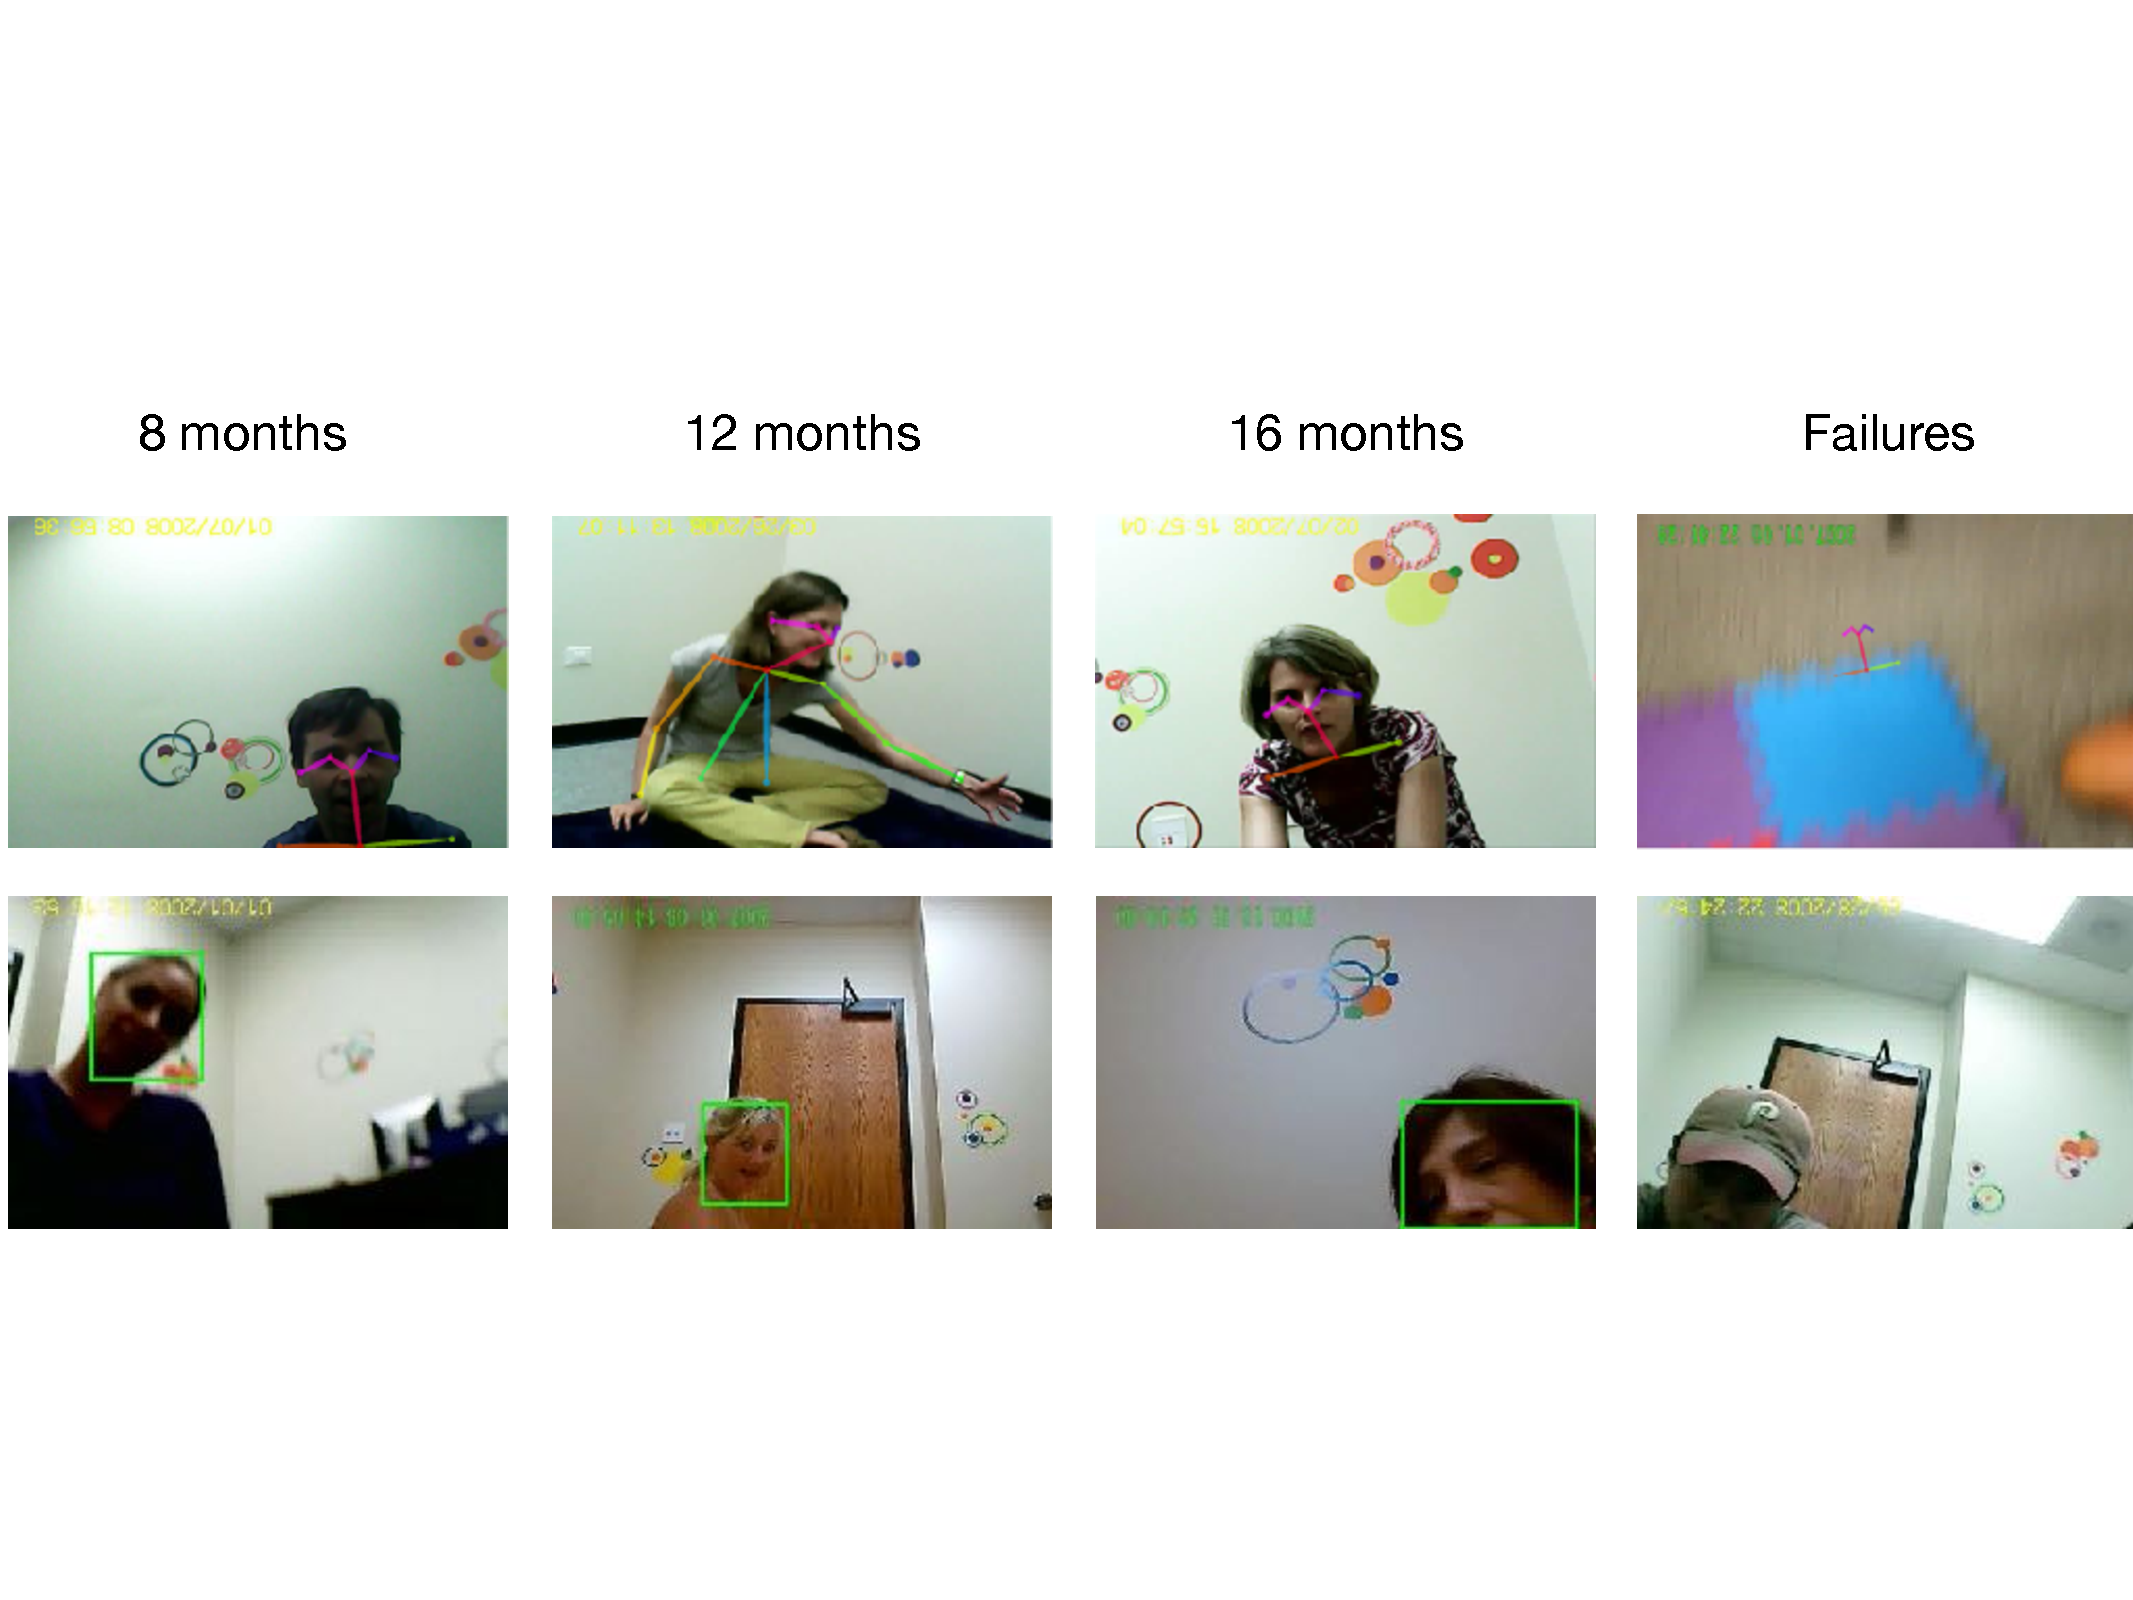
\includegraphics[width=6in]{images/detector_samples_banner.pdf}
\caption{\label{fig:frames} Example face and pose detections made by OpenPose (top row) and MTCNN (bottom row) from a child in each age group. The last column features a false positive from OpenPose and a false negative from MTCNN.}
\end{figure*}

Headcam videos were trimmed such that they excluded the instruction
phase when the experimenter was in the room and were automatically
synchronized with the tripod-mounted videos using FinalCut Pro Software.
These sessions yielded videos of 516 minutes (almost a milion frames),
with an average video length of 8.6 minutes (min = 4.53, max = 19.35).

\subsubsection{Posture and Orientation
Annotation}\label{posture-and-orientation-annotation}

We created a set of custom annotations that described the child's
physical posture (e.g.~standing) and the orientation of the caregiver
relative to the child (e.g.~far away). The child's posture was
categorized as being held/carried, prone (crawling or lying), sitting,
or standing. The caregiver's orientation was characterized as being
close to the child, far from the child, and behind the child
(independent of distance). For the first two annotations (close/far from
the child), the caregiver could either be to the the front or to the
side of the child. All annotations were made by a trained coder using
the OpenSHAPA/Datavyu software (K. Adolph, Gilmore, Freeman, Sanderson,
\& Millman, 2012), and times when the child was out of view of the
tripod camera were marked as uncodable and were excluded from these
annotations.

\subsection{Face and Hand Detection}\label{face-and-hand-detection}

We used three face detection systems to measure infants' changing access
to faces. The first of these is the most commonly-used and widely
available face detection algorithm: Viola-Jones. We used this as a
benchmark for performance, as while it can achieve impressive accuracy
in some situations, it is notoriously bad at dealing with occluded faces
(Scheirer, Anthony, Nakayama, \& Cox, 2014). We next capitalized tested
the performance of two face detectors that both made use of recently
developed Convolutional Neural Networks (CNNs) to extract face
information. The first algorithm was specifically optimized for face
detection, and the second algorithm was this to extract information
about the position of 18 different body parts. For the second algorithm
(called OpenPose) (Cao et al., 2017), we used the agent's nose (one of
the 18 body parts detected) to operationalize the presence of faces, as
any half of a face necessarily contains a nose.

The OpenPose detector also provided us with the location of an agent's
wrists, which we used as a proxy for the presence of a hand. We did so
first because we did not capture the entire visual field experienced by
the infants/children. Thus, even though the video may only show the
presence of a wrist, the caregiver's hand may be within the child's
field of view. Second, we did so because hands are often occluded by
objects when caregivers are interacting with children, yet still
visually accessible by the child and part of their joint interaction.
For example, if a caregiver was holding a toy and presenting it to the
infant, their wrists may be visible but their hand may not necessarily
be (as it is occluded by the toy).

\subsubsection{Algorithms}\label{algorithms}

The first face detection system made use of a series of Haar
feature-based cascade classifiers (Viola \& Jones, 2004) applied to each
individual frame. This detector provided information about the presence
of a face as well as its size and position. The second algorithm (based
on work by K. Zhang et al. (2016)) using multi-task cascaded
convolutional neural networks (MTCNNs). The system was built using a
novel cascaded CNN-based framework for joint detection and alignment,
built to perform well in real-world environments where varying
illuminations and occlusions are present. We used a Tensorflow
implementation of this algorithm provided by
(\url{https://github.com/davidsandberg/facenet}). Like Viola-Jones, this
detector provided information about the presence of a face as well as
its size and position.

The CNN-based pose detector (OpenPose (Cao et al., 2017; Simon, Joo,
Matthews, \& Sheikh, 2017; Wei, Ramakrishna, Kanade, \& Sheikh, 2016))
provided the locations of 18 body parts (ears, nose, wrists, etc.)
avaliable at
\url{https://github.com/CMU-Perceptual-Computing-Lab/openpose}. The
system uses a CNN for initial anatomical detection and subsequently
applies part affinity fields (PAFs) for part association, producing a
series of body part candidates. The candidates are then matched to a
single individual and finally assembled into a pose; here, we only made
use of the body parts relevant to the face and hands (nose and wrists).
We operationalized face detections as any frames containing a nose, and
hand detections as any frames containing either the left orright wrist.

\subsubsection{Detector evaluation}\label{detector-evaluation}

To evaluate face detector performance, we constructed an unbiased ``gold
set'' of labeled frames that accounted for the relatively rare
appearance of faces in the dataset. We thus hand-labeled two samples: a
sample containing a high density of faces (half reported by MTCNN, half
by OpenPose) and a random sample from the remaining frames. Each sample
was comprised of an equal number of frames taken from each child's
video. Faces were classifed as present in a frame if at least half of
the face was showing. Precision (hits / hits + false alarms), recall
(hits / hits + misses), and F-score (harmonic mean of precision and
recall) were calculated for all detectors and are reported in Table 2.
For wrist detections, the ``gold set'' was constructed in the same
manner, with the exception that frames with a high density of wrists
were taken by pose detections made by OpenPose.

For face detection, MTCNN outperformed OpenPose when taking into account
only the composite F-score (0.89 MTCNN vs.~0.83 OpenPose); we thus use
MTCNN detections in the following analyses. Although MTCNN and OpenPose
performed comparably with the random sample, MTCNN performed better on
the high density sample (specifically looking at precision), suggesting
that OpenPose generated more false positives than MTCNN. ViolaJones
performed quite poorly relative to the other detectors, especially with
respect to the random sample.

For wrist detection, OpenPose performed moderately well (F = 0.74) with
relatively high precision, but low recall on the randomly sampled set of
frames (see Table 2). We thus analyze wrist detections, with the caveat
that we are likely underestimating the proportion of wrists overall in
the datatset.

\begin{table}[ht]
\centering
\begin{tabular}{rllrrr}
  \hline
   Algorithm & Sample\ Type & P & R & F \\ 
  \hline
  MTCNN-Faces & High density & 0.89 & 0.92 & \textbf{0.90} \\ 
  MTCNN-Faces & Random & 0.94 & 0.62 & 0.75 \\ 
  OpenPose-Faces & High density & 0.78 & 0.93 & 0.84 \\ 
  OpenPose-Faces & Random & 0.72 & 0.80 & \textbf{0.76} \\ 
  ViolaJones-Faces & High density & 0.96 & 0.44 & 0.60 \\ 
  ViolaJones-Faces & Random & 0.44 & 0.38 & 0.41 \\ 
  OpenPose-Wrists & High density & 0.66 & 1.00 & 0.79 \\ 
  OpenPose-Wrists & Random & 0.88 & 0.29 & 0.43 \\ 
   \hline
\end{tabular}
\caption{Detector performance on both high density samples (where proportion of faces detected was high) and random samples (where frames were randomly selected). P, R, and F denote precision, recall, and F-score, respectively. Scores in bold are the highest F-scores for each sample type.} 
\end{table}

\section{Results}\label{results}

First, we report developmental shifts in infants' posture and their
orientation relative to their caregiver. Then, we explore how these
changes influence children's visual access to faces and wrists/hands
across this developmental time range. Finally, we explore how these
changes impact the accessibility of faces and wrists/hands during
labeling events.

\subsection{Changes in Posture and
Orientation}\label{changes-in-posture-and-orientation}

\begin{CodeChunk}
\begin{figure}[h]

{\centering \includegraphics{figs/posture-1} 

}

\caption[Proportion time that infants in each age group spent in each posture/orientation relative to their caregiver]{Proportion time that infants in each age group spent in each posture/orientation relative to their caregiver.}\label{fig:posture}
\end{figure}
\end{CodeChunk}

We noted characteristic changes in infants' posture and orientation
across this developmental time range. The proportion of time infants
spent sitting decreased with age, and the proportion of time infants
spent standing increased with age. Both 8 month-olds and 12 month-olds
spent equivalent amounts of time either lying/crawling, which was
markedly decreased in the 16-month-olds, who spent most of their time
either sitting or standing (see Figure \ref{fig:posture}). We also
observed characteristic changes in children's orientation relative to
their caregivers: the 8-month-olds spent more time with their caregiver
behind them supporting their sitting positions (see Figure
\ref{fig:posture}).

\subsection{Changes in Access to Faces and
Hands}\label{changes-in-access-to-faces-and-hands}

\begin{CodeChunk}
\begin{figure}[h]

{\centering \includegraphics{figs/detByAge-1} 

}

\caption[Proportion of faces detected by the MTCNN model (left) and wrists detected by the OpenPose model (right) as a function of child's age]{Proportion of faces detected by the MTCNN model (left) and wrists detected by the OpenPose model (right) as a function of child's age. Larger dots indicate children who had longer play sessions and thus for whom there was more data.}\label{fig:detByAge}
\end{figure}
\end{CodeChunk}\begin{CodeChunk}
\begin{figure*}[h]

{\centering \includegraphics{figs/detByPosOrient-1} 

}

\caption[Proportion face detections as a function of children's posture (top panel) and orientation (bottom panel), binned by the age of the participant]{Proportion face detections as a function of children's posture (top panel) and orientation (bottom panel), binned by the age of the participant.}\label{fig:detByPosOrient}
\end{figure*}
\end{CodeChunk}

We first examined the proportion of face and wrist detections across
age; a full summary can be seen in Figure \ref{fig:detByAge}. When
looking at face presence, we observed a slight U-shaped function both
when analyzing the output of the MTCNN and OpenPose detectors, such that
12-month-olds appeared to experience slighly fewer faces faces than 8 or
16-month-olds.

However, we found that any age related effects were much smaller
compared to the impact of postural and locomotive changes on children's
visual access to faces. Children's posture was a major factor both in
how many faces and wrists/hands they saw during the play session.
Infants who were sitting saw more faces than infants who were lying down
or being carried, while infants who were standing saw the most faces
(Figure \ref{fig:detByPosOrient}, upper panel); this same pattern was
also true for wrists/hand detectinos. We also examined how the child's
orientation relative to their caregiver impacted their visual access to
faces and hands. Children who were far away from their caregiver were
more likely to see faces than children who were close to their
caregiver; this was true within all age groups (Figure
\ref{fig:detByPosOrient}, lower panel).

\begin{table}[H]
\centering
\begin{tabular}{rrrrr}
  \hline
 & Estimate & Std. Error & z value & Pr($>$$|$z$|$) \\ 
  \hline
Intercept & -5.2469 & 0.0584 & -89.88 & 0.0000 \\ 
  Age & 0.0847 & 0.0041 & 20.89 & 0.0000 \\ 
  Prone & 0.2015 & 0.0564 & 3.57 & 0.0004 \\ 
  Sit & 1.4053 & 0.0541 & 25.98 & 0.0000 \\ 
  Stand & 1.4272 & 0.0542 & 26.33 & 0.0000 \\ 
  Close & 1.8239 & 0.0230 & 79.17 & 0.0000 \\ 
  Far & 2.5479 & 0.0239 & 106.42 & 0.0000 \\ 
   \hline
\end{tabular}
\caption{Model coefficients from a generalized linear model predicting the proportion of faces seen by infants.} 
\end{table}

\begin{table}[H]
\centering
\begin{tabular}{rrrrr}
  \hline
 & Estimate & Std. Error & z value & Pr($>$$|$z$|$) \\ 
  \hline
Intercept & -5.0818 & 0.0776 & -65.46 & 0.0000 \\ 
  Age & 0.0564 & 0.0050 & 11.35 & 0.0000 \\ 
  Prone & 0.9499 & 0.0774 & 12.27 & 0.0000 \\ 
  Sit & 1.7282 & 0.0758 & 22.79 & 0.0000 \\ 
  Stand & 1.6618 & 0.0760 & 21.88 & 0.0000 \\ 
  Close & 0.7472 & 0.0188 & 39.81 & 0.0000 \\ 
  Far & 1.6357 & 0.0200 & 81.61 & 0.0000 \\ 
   \hline
\end{tabular}
\caption{Model coefficients from a generalized linear model predicting the proportion of wrists seen by infants.} 
\end{table}

To formalize these observations, we fit a generalized linear model to
the proportion of faces infants saw in each posture and orientation (as
detected by MTCNN), with participant's age, orientation, and posture as
independent variables. A summary of the coefficients of a model with
only main effects (and no interactions) model can be found in Table 3.
When we did include interaction terms between age, posture, and
orientation, age no longer remained a significant predictor (b = -15.84,
SE = 113.98, z = -0.14 , p = 0.89). We also found the same pattern with
respect to infant's visual access to hands (see Table 4); including
interaction terms also eliminated any main effect of age on the
proportion of hands detected (b = -15.7, SE = 113.98, z = -0.14, p =
0.89). Thus, these results suggest that infants' access to social
information is heavily influenced by their postural and locomotive
developments.

\begin{CodeChunk}
\begin{figure}[H]

{\centering \includegraphics{figs/detByNaming-1} 

}

\caption[Proportion face detections around a naming instance ('Look, a Zem']{Proportion face detections around a naming instance ('Look, a Zem'; +/- 2 seconds around each utterance) as a function of infants' posture.}\label{fig:detByNaming}
\end{figure}
\end{CodeChunk}

\subsection{Access to Faces and Hands During Labeling
Events}\label{access-to-faces-and-hands-during-labeling-events}

Finally, we analyzed how face and wrist/hand detections changed during
object labeling events as a function of infant's posture and
orientation. Specfically, we analyzed a four-second window around each
labeling event (e.g., ``Look at the {[}zem{]}!''); these labeling events
were hand-annotated and automatically synchronized with the
frame-by-frame face detections. We found that infants' posture and
orientations impacted the degree to which they saw their caregiver's
face and wrist during a labeling event; infants who were sitting or
standing were more likely to have access to this social information.
However, this did not manifest in a direct change the presence of
wrists/hands before vs.~after naming events (average difference in
proportion of wrists detected, 8 m.o. = -0.006, 12 m.o. = -0.013, 16
m.o. = -0.007) or in proportion of faces detected (average difference in
proportion of faces detected, 8 m.o. = -0.002, 12 m.o. = 0, 16 m.o. =
-0.004).

\section{General Discussion}\label{general-discussion}

We used a head-mounted camera to explore how children's postural and
locomotive development directly impacts their access to social
information, here operationalized as the presence of the faces and
wrists of their caregiver. We found that children's posture and
orientation towards their caregiver changed systematically across age,
and that both of these factors dramatically impacted the proportion of
faces and wrists/hands that were available in the child's visual field.
Thus, infants' postural and locomotive developments are mediating
factors that explain some of the age-related changes in the proportion
of faces and wrists/hands that are visually available to infants.
Broadly, this work suggests that motoric developments mediate how
infants experience their visual world and the social information in it:
infants that are sitting and standing have a different view of their
world, the people in it, and the actions that are being performed.

This work also deploys novel advancements in computer vision to the
study of developmental psychology. The field of object detection and
recognition has advanced dramatically in the past five years since the
re-birth of deep learning algorithms (Krizhevsky, Sutskever, \& Hinton,
2012), creating a new generation of algorithmic tools. These tools are
substantially better equipped to deal with noisier, more complicated
datasets and can extract richer and more detailed information. Videos
from the infant perspective provided substantial challenges (e.g.,
partially occluded faces) for the classic models of face detection
(e.g., ViolaJones) (Viola \& Jones, 2004). Further, as the headcam
technologies employed here were inexpensive and the computer vision
algorithms freely available, this method is a promising avenue for
quantifying the visual and social information available to infant
learners.

Broadly, we suggest that the combined use of these new tools can be
leveraged to understand the changing infant perspective on the visual
world and the implications of these changes for linguistic, cognitive,
and social development.

\section{Acknowledgements}\label{acknowledgements}

Thanks to Kaia Simmons, Kathy Woo, Aditi Maliwal, and other members of
the Language and Cognition Lab for help in recruitment, data collection,
and annotation. This research was supported by a John Merck Scholars
grant to MCF. An earlier version of this work was presented to the
Cognitive Science Society in Frank et al. (2013). Please address
correspondence to Michael C. Frank, Department of Psychology, Stanford
University, 450 Serra Mall (Jordan Hall), Stanford, CA, 94305, tel:
(650) 724-4003, email: \texttt{mcfrank@stanford.edu}.

\section{References}\label{references}

\setlength{\parindent}{-0.1in} \setlength{\leftskip}{0.125in} \noindent

\hypertarget{refs}{}
\hypertarget{ref-adolph2007}{}
Adolph, K., \& Berger, S. (2007). Motor development. In \emph{Handbook
of child psychology}. Wiley Online Library.

\hypertarget{ref-adolph2012}{}
Adolph, K., Gilmore, R., Freeman, C., Sanderson, P., \& Millman, D.
(2012). Toward open behavioral science. \emph{Psychological Inquiry},
\emph{23}(3), 244--247.

\hypertarget{ref-bambach2017}{}
Bambach, S., Crandall, D. J., Smith, L. B., \& Yu, C. (2017). An
egocentric perspective on active vision and visual object learning in
toddlers. In \emph{Proceedings of the seventh joint ieee conference on
development and learning and on epigenetic robotics}.

\hypertarget{ref-cao2017realtime}{}
Cao, Z., Simon, T., Wei, S.-E., \& Sheikh, Y. (2017). Realtime
multi-person 2D pose estimation using part affinity fields. In
\emph{CVPR}.

\hypertarget{ref-clerkin2017}{}
Clerkin, E. M., Hart, E., Rehg, J. M., Yu, C., \& Smith, L. B. (2017).
Real-world visual statistics and infants' first-learned object names.
\emph{Phil. Trans. R. Soc. B}, \emph{372}(1711), 20160055.

\hypertarget{ref-csibra2009natural}{}
Csibra, G., \& Gergely, G. (2009). Natural pedagogy. \emph{Trends in
Cognitive Sciences}, \emph{13}(4), 148--153.

\hypertarget{ref-cummings1988}{}
Cummings, M., Van Hof-Van Duin, J., Mayer, D., Hansen, R., \& Fulton, A.
(1988). Visual fields of young children. \emph{Behavioural and Brain
Research}, \emph{29}(1), 7--16.

\hypertarget{ref-farroni2002eye}{}
Farroni, T., Csibra, G., Simion, F., \& Johnson, M. H. (2002). Eye
contact detection in humans from birth. \emph{Proceedings of the
National Academy of Sciences}, \emph{99}(14), 9602--9605.

\hypertarget{ref-fausey2016}{}
Fausey, C. M., Jayaraman, S., \& Smith, L. B. (2016). From faces to
hands: Changing visual input in the first two years. \emph{Cognition},
\emph{152}, 101--107.

\hypertarget{ref-franchak2011}{}
Franchak, J., Kretch, K., Soska, K., \& Adolph, K. (2011). Head-mounted
eye tracking: A new method to describe infant looking. \emph{Child
Development}.

\hypertarget{ref-frank2014visual}{}
Frank, M. C., Amso, D., \& Johnson, S. P. (2014). Visual search and
attention to faces during early infancy. \emph{Journal of Experimental
Child Psychology}, \emph{118}, 13--26.

\hypertarget{ref-frank2013}{}
Frank, M. C., Simmons, K., Yurovsky, D., \& Pusiol, G. (2013).
Developmental and postural changes in children’s visual access to faces.
In \emph{Proceedings of the 35th annual meeting of the cognitive science
society} (pp. 454--459).

\hypertarget{ref-frank2012measuring}{}
Frank, M. C., Vul, E., \& Saxe, R. (2012). Measuring the development of
social attention using free-viewing. \emph{Infancy}, \emph{17}(4),
355--375.

\hypertarget{ref-gredeback2010development}{}
Gredebäck, G., Fikke, L., \& Melinder, A. (2010). The development of
joint visual attention: A longitudinal study of gaze following during
interactions with mothers and strangers. \emph{Developmental Science},
\emph{13}(6), 839--848.

\hypertarget{ref-gredeback2008microstructure}{}
Gredebäck, G., Theuring, C., Hauf, P., \& Kenward, B. (2008). The
microstructure of infants' gaze as they view adult shifts in overt
attention. \emph{Infancy}, \emph{13}(5), 533--543.

\hypertarget{ref-iverson2010}{}
Iverson, J. M. (2010). Developing language in a developing body: The
relationship between motor development and language development.
\emph{Journal of Child Language}, \emph{37}(2), 229--261.

\hypertarget{ref-karasik2014}{}
Karasik, L. B., Tamis-LeMonda, C. S., \& Adolph, K. E. (2014). Crawling
and walking infants elicit different verbal responses from mothers.
\emph{Developmental Science}, \emph{17}(3), 388--395.

\hypertarget{ref-kretch2014}{}
Kretch, K. S., Franchak, J. M., \& Adolph, K. E. (2014). Crawling and
walking infants see the world differently. \emph{Child Development},
\emph{85}(4), 1503--1518.

\hypertarget{ref-krizhevsky2012imagenet}{}
Krizhevsky, A., Sutskever, I., \& Hinton, G. E. (2012). Imagenet
classification with deep convolutional neural networks. In
\emph{Advances in neural information processing systems} (pp.
1097--1105).

\hypertarget{ref-mayer1988}{}
Mayer, D., Fulton, A., \& Cummings, M. (1988). Visual fields of infants
assessed with a new perimetric technique. \emph{Investigative
Ophthalmology \& Visual Science}, \emph{29}(3), 452--459.

\hypertarget{ref-meltzoff2007like}{}
Meltzoff, A. N. (2007). ``Like me'': A foundation for social cognition.
\emph{Developmental Science}, \emph{10}(1), 126--134.

\hypertarget{ref-scheirer2014perceptual}{}
Scheirer, W. J., Anthony, S. E., Nakayama, K., \& Cox, D. D. (2014).
Perceptual annotation: Measuring human vision to improve computer
vision. \emph{IEEE Transactions on Pattern Analysis and Machine
Intelligence}, \emph{36}(8), 1679--1686.

\hypertarget{ref-simon2017hand}{}
Simon, T., Joo, H., Matthews, I., \& Sheikh, Y. (2017). Hand keypoint
detection in single images using multiview bootstrapping. In
\emph{CVPR}.

\hypertarget{ref-viola2004robust}{}
Viola, P., \& Jones, M. J. (2004). Robust real-time face detection.
\emph{International Journal of Computer Vision}, \emph{57}(2), 137--154.

\hypertarget{ref-walle2014}{}
Walle, E. A., \& Campos, J. J. (2014). Infant language development is
related to the acquisition of walking. \emph{Developmental Psychology},
\emph{50}(2), 336.

\hypertarget{ref-wei2016cpm}{}
Wei, S.-E., Ramakrishna, V., Kanade, T., \& Sheikh, Y. (2016).
Convolutional pose machines. In \emph{CVPR}.

\hypertarget{ref-yoshida2008}{}
Yoshida, H., \& Smith, L. (2008). What's in view for toddlers? Using a
head camera to study visual experience. \emph{Infancy}, \emph{13},
229--248.

\hypertarget{ref-yurovsky2012}{}
Yurovsky, D., Smith, L., \& Yu, C. (in press). Statistical word learning
at scale: The baby's view is better. \emph{Developmental Science}.

\hypertarget{ref-zhang2016}{}
Zhang, K., Zhang, Z., Li, Z., \& Qiao, Y. (2016). Joint face detection
and alignment using multitask cascaded convolutional networks.
\emph{IEEE Signal Processing Letters}, \emph{23}(10), 1499--1503.

\end{document}
